\section{The Plant}
In order to properly understand and control the P\&T system, mathematical models for the pan and tilt systems (the plant) had to be developed. This section will discuss the process of initially testing for relevant DC motor data, the derivation of a mathematical model, then comparing this  model to the test data for validation of its accuracy. Finally, the same method will be used to develop models for the behaviour of the pan and tilt systems as a whole.

\subsection{DC Motor Modelling}
\subsubsection{DC Motor Tests}
The purpose of these tests are to analyse and generate a blackbox model for the DC motor, based on its step response. 

The motor was set up with a switch connected to a power supply set at the desired voltage to test. This would create a physical step response from the motor when the switch was toggled. The two encoders output on the EMG30 are open collectors, so the outputs were connected to pull-up resistance to produce a desired signal. The pull-up resistors for these tests were picked to be around 300 ohm.

An oscilloscope was set to measure the two encoder outputs on their own individual channels. The sampling starts on an edge trigger with a sampling rate of 2 MHz and stops the sampling after 0.5 seconds.
These 2 set of samples would together be the data defining an step response.

Following step responses were sampled(Figure \ref{fig:stepresponses1to12V}), and the information extracted (Figure \ref{fig:StepResponseData}) from the data was calculated in matlab. 
% Optional reference to actual matlab data if we want and add it to CD.

\begin{figure}[h!]
\centering
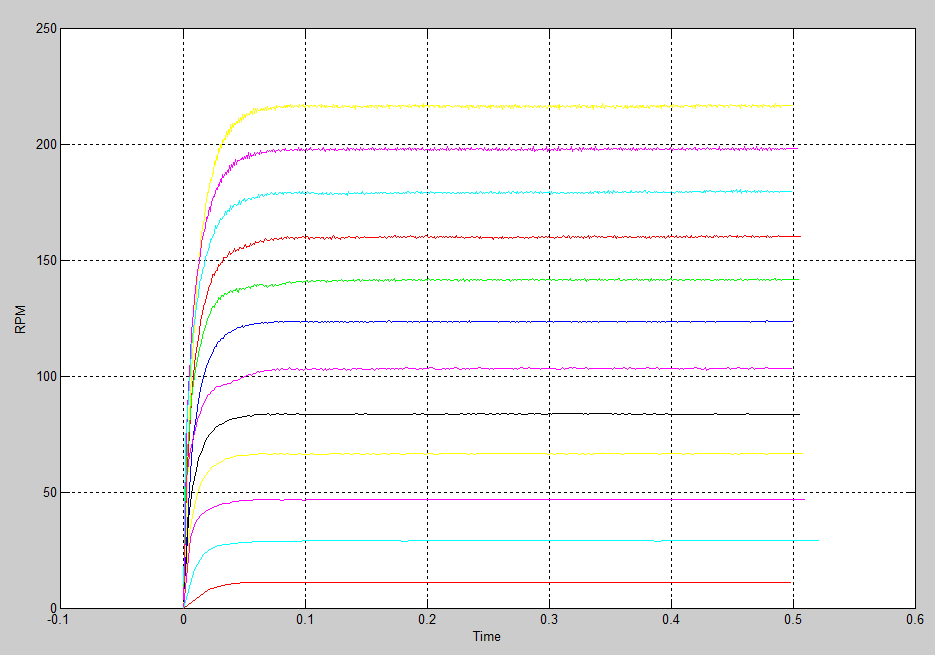
\includegraphics[scale=0.4]{Billeder/Stepresponses1to12V.png}
\caption{DC motor step responses from 1 to 12V. The bottom red line is 1V, and the upper yellow line is 12V}
\label{fig:stepresponses1to12V}
\end{figure}

\begin{figure}[h!]
\centering
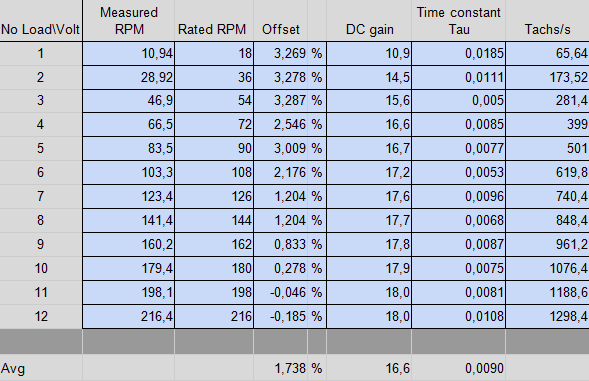
\includegraphics[scale=0.7]{Billeder/StepResponseData}
\caption{Table summarizing the information from the DC motor tests.}
\label{fig:StepResponseData}
\end{figure}

As noted, the step responses of the motor appear to be of a first-order linear-time-invariant (LTI) system. This means the system can be estimated as:

\begin{equation}
DCgain\frac{1}{\tau s+1}
\end{equation}

The DC gain is the steady state value divided by the steady state (constant) value of the input step.

\begin{equation}
\frac{216}{12V}=18\frac{rpm}{V}
\end{equation}

This indicates that RPM is directly proportional to a voltage. The expected proportionality (in blue) is plotted below together with the actual measured RPM (in green) in figure \ref{fig:RPMLinearityAnalysis}.

\begin{figure}[h!]
\centering
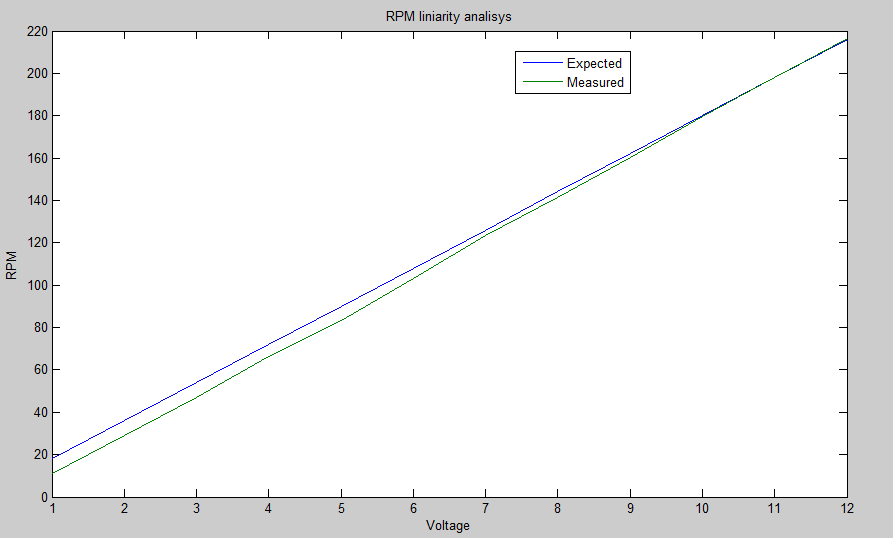
\includegraphics[scale=0.4]{Billeder/RPMLinearityAnalysis.png}
\caption{Comparing measured RPM values to expected ones}
\label{fig:RPMLinearityAnalysis}
\end{figure}

As seen, the actual RPM of the motor is not directly proportional to a voltage, but the difference is at max a 3.287\% offset from the expected. Since this is relatively low, the system is estimated to be proportional. Though at low voltages the relative DC gain at that voltage starts to differ significantly from the estimated values. Therefore the DC gain is estimated as the mean value of the actual DC gains measured for the voltages 4V to 12V, since the DC gain in this range is relatively linear. The DC gain is: $\approx 17.6\frac{rpm}{V}$

The time constant tau is the time when the step response reaches $1-1/e\approx63.2\%$ of its final value. This time constant is expected to be constant, but as seen in figure \ref{fig:TimeConstantLinearityAnalysis}, at low voltages there seems to be some uncertainties regarding the time constant.

\begin{figure}[h!]
\centering
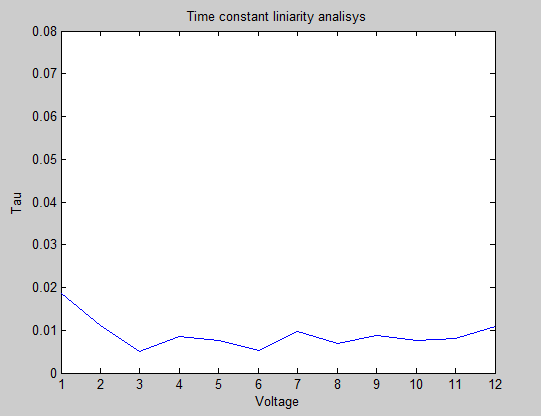
\includegraphics[scale=0.5]{Billeder/TimeConstantLinearityAnalysis.png}
\caption{Time constant for the DC Motor at different voltages}
\label{fig:TimeConstantLinearityAnalysis}
\end{figure}

This behavior can be explained by variations in the actual experiments, since the encoders are not uniformly placed in the motor. The start position of the encoders can have some impact regarding the experimental results. Other than that, it would be expected to see some differences from the lower voltages compared to the higher, since the DC gain of the system indicated some nonlinearity. The time constant, Tau, is then estimated to be the mean value from 1 to 12 volts, $\tau\approx0.009 seconds$.

The transfer function for the DC motor is therefore now defined as follows:

\begin{equation}
G(s)=\frac{17.6}{0.009s+1}
\end{equation}

As seen on Figure \ref{fig:FirstOrderApproximation} the first-order approximation G(s) of the motor is relatively accurate.

\begin{figure}[h!]
\centering
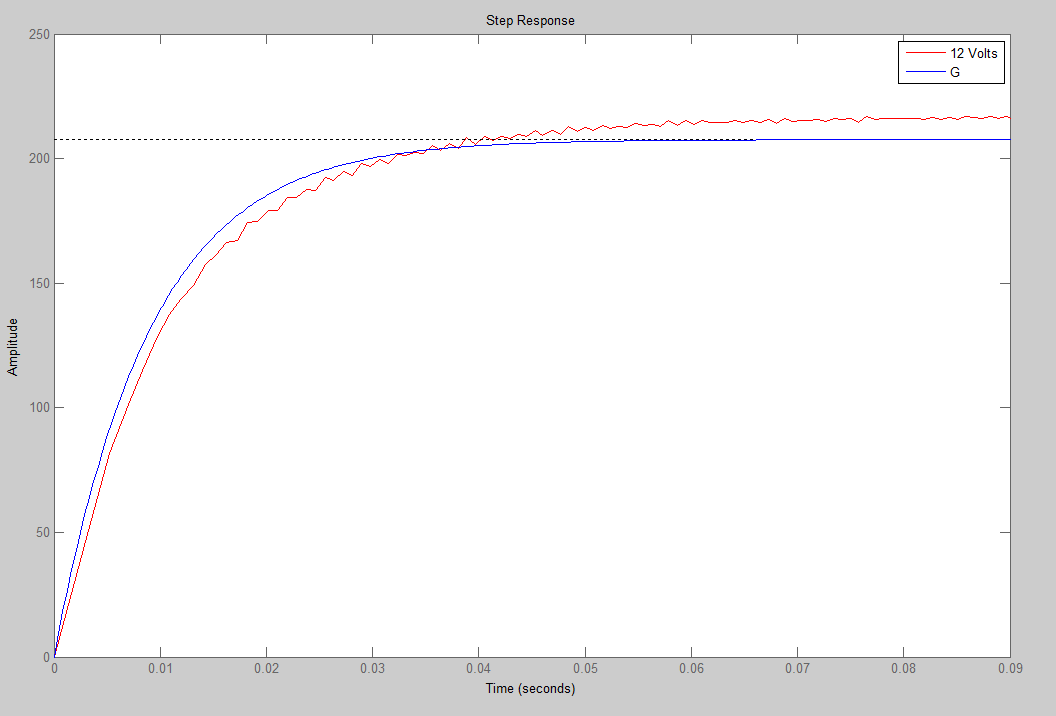
\includegraphics[scale=0.35]{Billeder/FirstOrderApproximation.png}
\caption{Comparation of the first order approximation step response and the actual step response from research.}
\label{fig:FirstOrderApproximation}
\end{figure}

\subsubsection{Discussion}
Having modelled our DC-motor as a first order LTI system, it is relevant to discuss the reliability and accuracy of this model. In reality, the transfer function for the motor includes both an external, mechanical part and an internal, electrical part (the armature).\footnote{Model and transfer function from Control Systems: Twelfth Edition p. 72}

\begin{equation}
\frac{\theta(s)}{V_f (s)}=G(s)=\frac{K_m / (bR_f)}{s(\tau_f s+1)(\tau_L s+1)}
\end{equation}

This model is actually a second order system. However the time constant $\tau_f$, denoting the response time of the internal electronics of the motor, is usually negligible compared to the mechanical dynamics of the motor\footnote{Modern Control Systems: Twelfth Edition p72}. This makes sense both intuitively and mathematically, as the relatively faster armature with an associated pole further away from origin will have less of an impact on the overall system response, and can thus be omitted for the sake of simplicity. Typical values for these time constants show this aswell.

The first and second order transfer functions generated using these time constants are close to identical, as can be seen in figure \ref{fig:1st2ndorderstep}. The motor constants used:

Field time constant: $\tau_f = 1ms$ 

Rotor time constant\footnote{Modern Control Systems: Twelfth edition p77.}: $\tau = 100ms$ 

\begin{figure}[h!]
\centering
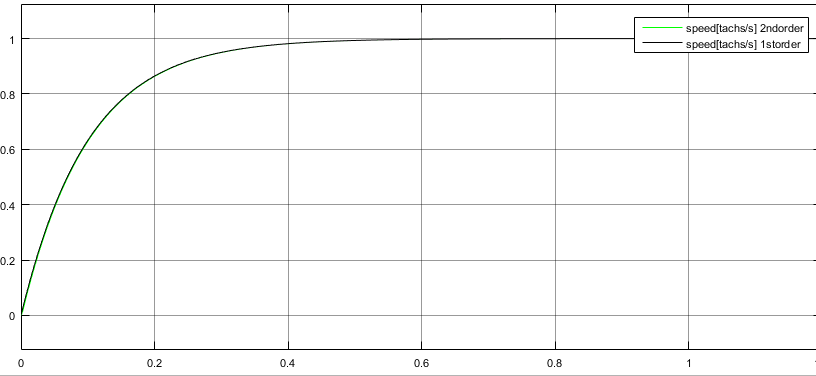
\includegraphics[scale=0.6]{Billeder/1st2ndorderstep.png}
\caption{Comparing 1st and 2nd order transfer function step responses. x-axis: sec, y-axis: normalized DC gain}
\label{fig:1st2ndorderstep}
\end{figure}

Omitting the armature from the derived transfer function gives us the following, which essentially equals our first order estimation. This indicates that a first order approximation of the motor can be very accurate, while simultaneously simplifying the controller design process.

\begin{equation}
\frac{K_m /(R_a b+K_b K_m )}{s(\tau_1 s +1)}
\end{equation}

\subsubsection{SI-units for DC Gain}
Looking at the model in the larger context of our control system, it is evident that using $RPM/V$ as the SI-unit for DC-gain is less than optimal. The feedback from the Hall sensors is in the form of tachs, and would thus require a conversion in order to be interpreted as motor rotations. In addition to that, the controlled variable of our system is the position of the motor in terms of tachs. The transfer function can easily be modified to reflect this through an integration, effectively making our transfer function a second order system.

Speed:
\begin{equation}
G(s)=\frac{105.6}{0.009s+1} \frac{[tachs/sec]}{[V]}
\end{equation}

Position:
\begin{equation}
G(s)=\frac{105.6}{0.009s^2+s} \frac{[tachs/sec]}{[V]}
\label{eq:PosTF}
\end{equation}

The behavior of these transfer functions given a step input can be seen in figure \ref{fig:SpeedPosSim12V}. This behavior looks very promising. The speed transfer function step response shows an acceleration, until the speed reaches the $DC Gain * 12V$. The position transfer function also behaves as expected, as the area below the speed transfer function. 

\begin{figure}[h!]
\centering
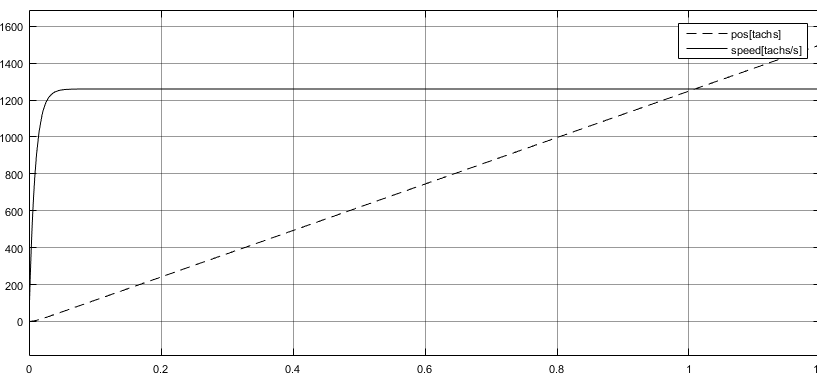
\includegraphics[scale=0.6]{Billeder/SpeedPosSim12V.png}
\caption{speed \& position simulation given a 12V input.}
\label{fig:SpeedPosSim12V}
\end{figure}

\subsection{P\&T System Modelling}
Having modelled the DC motor, it is now time to move on to the modelling of the entire plant. The same methods will be used, except now we are testing and considering the P\&T loads and their influence on the system.

\subsubsection{Inertia in the P\&T system}
Because of inertia present in the P\&T system parts, it can be expected that the constants of the individual motors will look different than those describing the motor without load. Also, because transfer function of the DC motor without load is approximated to be linear, we assume the same from the specific transfer functions of the P\&T motors.

\subsubsection{Tests of the P\&T motors}
Step response tests were applied to the motors on the actual P\&T system. Because of restrictions on the pan part of the system, voltages tested ranged from 3V to 8V. The data has been analysed to find values of constants related to the method of approximating a plant of a DC motor (Figure \ref{fig:PanTiltStepDataTable}).

\begin{figure}[h!]
\centering
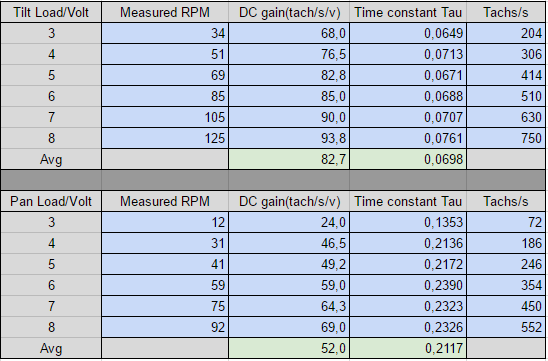
\includegraphics[scale=0.6]{Billeder/PanTiltStepDataTable.png}
\caption{Table of P\&T step response data}
\label{fig:PanTiltStepDataTable}
\end{figure}

As seen below in figure \ref{fig:PTStepResponseGraph}, the step response spikes at first. It is assumed this spike occurs primarily because of the following:

In the gear network connecting the actual motor and the pan or tilt part, there are small gaps between individual teeth. The motor is then switched on and while the collective gap closes, the motor runs as if it had no inertia. When the gap is closed the motor is slowed drastically because of the inertia of the pan or tilt part. 

The two things together create the spike we see on figure \ref{fig:PTStepResponseGraph} below. Because we assume linearity of the actual systems, we disregard the spike and look at the graphs after the spike has ended to find Tau.

\begin{figure}[h!]
\centering
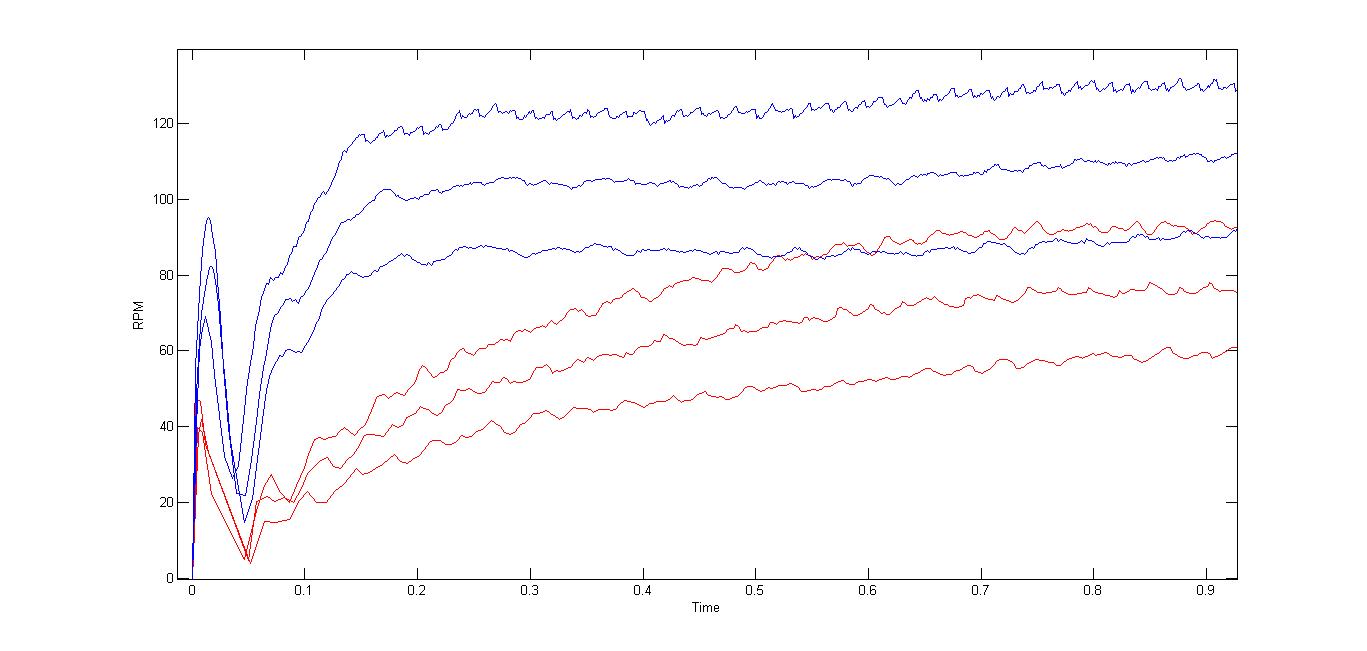
\includegraphics[scale=0.35]{Billeder/PTStepResponseGraph.png}
\caption{The P\&T response to 6V-7V-8V. Blue: Tilt, Red: Pan}
\label{fig:PTStepResponseGraph}
\end{figure}

Applying the method for creating a plant for a DC motor, discussed earlier, the actual constants for the pan and tilt systems are used in this context to create dedicated transfer functions for each motor in the P\&T system. The plants can be seen as equation \ref{eq:Gpan} for the pan part and equation \ref{eq:Gtilt} for the tilt part:

\begin{equation}
G_{pan} (s) = \frac{52}{0.212s+1}\frac{[tachs/sec]}{[V]}
\label{eq:Gpan}
\end{equation}

\begin{equation}
G_{tilt} (s) = \frac{82.7}{0.07s+1}\frac{[tachs/sec]}{[V]}
\label{eq:Gtilt}
\end{equation}

\subsection{Overview}
The mathematical models necessary for predicting and controlling P\&T system behavior were found. It was found that a first order approximation was sufficient for modelling the system behavior, because of the negligible armature. Finding proper transfer functions for the P\&T systems posed a greater challenge than for the DC motor itself, because of unlinear behavior associated with the gear network in the system. Should an attempt be made to improve the models in the future, this would be an obvious place to begin. These models could be improved either through new tests that try to minimize the unlinearity, or through improvements in the analysis of the data.